\documentclass{article}

% if you need to pass options to natbib, use, e.g.:
%     \PassOptionsToPackage{numbers, compress}{natbib}
% before loading neurips_2025

% The authors should use one of these tracks.
% Before accepting by the NeurIPS conference, select one of the options below.
% 0. "default" for submission
\usepackage[main,final]{neurips_2025}
% the "default" option is equal to the "main" option, which is used for the Main Track with double-blind reviewing.
% 1. "main" option is used for the Main Track
% 2. "position" option is used for the Position Paper Track
%  \usepackage[position]{neurips_2025}
% 3. "dandb" option is used for the Datasets & Benchmarks Track
 % \usepackage[dandb]{neurips_2025}
% 4. "creativeai" option is used for the Creative AI Track
%  \usepackage[creativeai]{neurips_2025}
% 5. "sglblindworkshop" option is used for the Workshop with single-blind reviewing
 % \usepackage[sglblindworkshop]{neurips_2025}
% 6. "dblblindworkshop" option is used for the Workshop with double-blind reviewing
%  \usepackage[dblblindworkshop]{neurips_2025}
% After being accepted, the authors should add "final" behind the track to compile a camera-ready version.
% 1. Main Track
 % \usepackage[main, final]{neurips_2025}
% 2. Position Paper Track
%  \usepackage[position, final]{neurips_2025}
% 3. Datasets & Benchmarks Track
 % \usepackage[dandb, final]{neurips_2025}
% 4. Creative AI Track
%  \usepackage[creativeai, final]{neurips_2025}
% 5. Workshop with single-blind reviewing
%  \usepackage[sglblindworkshop, final]{neurips_2025}
% 6. Workshop with double-blind reviewing
%  \usepackage[dblblindworkshop, final]{neurips_2025}
% Note. For the workshop paper template, both \title{} and \workshoptitle{} are required, with the former indicating the paper title shown in the title and the latter indicating the workshop title displayed in the footnote.
% For workshops (5., 6.), the authors should add the name of the workshop, "\workshoptitle" command is used to set the workshop title.
% \workshoptitle{WORKSHOP TITLE}

% "preprint" option is used for arXiv or other preprint submissions
 % \usepackage[preprint]{neurips_2025}

% to avoid loading the natbib package, add option nonatbib:
%    \usepackage[nonatbib]{neurips_2025}

\usepackage[utf8]{inputenc} % allow utf-8 input
\usepackage[T1]{fontenc}    % use 8-bit T1 fonts
\usepackage{hyperref}       % hyperlinks
\usepackage{url}            % simple URL typesetting
\usepackage{booktabs}       % professional-quality tables
\usepackage{amsfonts}       % blackboard math symbols
\usepackage{nicefrac}       % compact symbols for 1/2, etc.
\usepackage{microtype}      % microtypography
\usepackage{xcolor}         % colors
\usepackage{enumitem}
\usepackage{graphicx}


% Note. For the workshop paper template, both \title{} and \workshoptitle{} are required, with the former indicating the paper title shown in the title and the latter indicating the workshop title displayed in the footnote. 
\title{Understanding conversation dynamics\\NLP analysis of sentiment, language and interruptions in podcasts}


% The \author macro works with any number of authors. There are two commands
% used to separate the names and addresses of multiple authors: \And and \AND.
%
% Using \And between authors leaves it to LaTeX to determine where to break the
% lines. Using \AND forces a line break at that point. So, if LaTeX puts 3 of 4
% authors names on the first line, and the last on the second line, try using
% \AND instead of \And before the third author name.


\author{
  Mikkel Vestergaard Devantier\\
  Computer Science student\\
  Aarhus Universitet\\
  \texttt{201905653} \\
  \And
  Nicoline Sørensen\\
  Data Science student\\
  Aarhus Universitet\\
  \texttt{202009037} \\
  \And
  Marcus Kjærgaard Olesen\\
  Data Science student\\
  Aarhus Universitet\\
  \texttt{202106575}\\
}


\begin{document}


\maketitle

\begin{abstract}
  Fill in abstract
\end{abstract}


\section{Introduction}
Podcasts are becoming increasingly popular as a form of entertainment for the general population, but the world of Natural Language Processing (NLP) they are especially interesting due to their loose and unstructured conversational format ranging from monologues to multi-speaker discussions. This makes podcasts interesting for NLP analysis, since we can look not only at the spoken content but also at other dimensions to shed light on timing, speakers, overlap and tune of the speakers throughout the conversation. Furthermore, podcasts are a great reflection of the messiness of real-world conversation, so the understanding of conversational dynamics in podcasts will also have broader use and value.

In this report we will dive into the analysis of conversational dynamics in podcasts across different genres through 3 different lenses, namely interruptions, sentiment and calls to action. By analyzing the conversational dynamics in three ways and combining the results, we aim to shed light on how these dynamics differ across different genres of podcasts.

Specifically, we work towards answering the following research questions:
\begin{itemize}
    \item [\textbf{RQ1:}] How does the polarity and intensity of sentiment evolve over the course of an episode, and how does it differ by genre?
    \item [\textbf{RQ2:}] How do patterns of interruptions differ across genres?
    \item [\textbf{RQ3:}] How does the frequncy and timing of calls to action differ by genre?
    \item [\textbf{RQ4:}] What is the nature of the relationships between sentiment, interruptions and calls to action?
\end{itemize}

\section{Data}
The dataset used in this analysis is the Structured Podcast Open Research Corpus (SPORC), which is a large multi-modal podcasts dataset containing transcriptions, speaker-turns, speaker information, genres and temporal information. The dataset consists of three levels of data; podcast-, episode- and turn level. The podcast level contains podcast wide metadata and is a collection of episodes. Meanwhile, the episode level data contains metadata on the episode like title, genre, speakers among others, while the turn level data consists of the transciption divided into turns along with the speaker label, start- and end time, duration etc.

To prepare the data for use, we had to establish a preprocessing pipeline to performing cleaning, filtering and decomposition of the data to support the subsequent analysis. We have chosen to only work with the podcast episodes in the 10,000 episode sample provided in the dataset due to the large size of the full dataset, since the analysis detailed in this report serves only as an indicator of potentially interesting findings, not conclusive evidence of such.

Upon loading the sample the dataset, we filter on the portion of the episodes containing one or more speaker turns, since the existence of turns deliver the temporal information and speaker labels used for analysis. The relevant set of episodes are transformed to a dataframe with the relevant attributes, and an additional dataframe stores the turns associated with these episodes along with additional properties related to the cleaning of the turns textual content. These turns are split into singular sentences to be used as the unit of analysis for the call to action and sentiment analysis, which is then aggregated back to turn- and episode level results for reporting, visualization and comparison purposes.

In working with the dataset we discovered a number of issues, which affects the analysis. Among others it is observed that multiple back to back turns are labeled as the same speaker, podcasts listed to have no guests sometimes have multiple speaker labels and a large number of turns consist of only a few words. These issues suggest quality issues in the automated inference of metadata using e.g. NER and heuristics, which should be accounted for when trying to conclude on the results on the performed analysis.

\section{Methods}
This section will detail the methodological approach to performing the analysis with the aim of answering the posed research questions. 

\subsection{Sentiment analysis}
To investigate the tone of the conversations, we perform sentiment analysis at the sentence level before aggregating results to turn, episode and genre levels. Sentiment can be quantified in different ways depending on the approach, but for this analysis the focus is on the polarity of the conversations, i.e. if the statements are positive, negative or neutral. Due to the time and resource constraints associated with this project it has not been possible to create an annotated set of correct labels for direct evaluations. Instead, we have chosen to use and compare two fundamentally different approaches to polarity classification to test the level of agreement as an informal robustness check.
\begin{enumerate}[leftmargin=*]

\item \textbf{DistilBERT} is a transformer based classifier finetuned on the SST-2 sentiment benchmark consisting of movie reviews. This model outputs a polarity label along with a confidence score for each sentence. These are combined in a single weighted score to allow for quantitative comparison. 

\item \textbf{VADER} on the other hand is a lexicon based sentiment classifier designed for shorter and more informal pieces of text. Vader outputs a continues score containing both polarity and intensity at once. 
\end{enumerate}

The two methods differ in their leverage of contextual information, their ideal text complexity and lenght and sensitivity to domain mismatches, which makes them interesting to compare on a dataset not ideally suited for either original domain. If a large degree of agreement is observed e.g. at the genre level our confidence in the results will increase even in the absence of formal accuracy evaluations of each method.

Beyond assigning polarity scores to the data and comparing agreement, we also wish to investigate these patterns and the method performance. The sentence level polarity is aggregated to turn and episode levels, which allow us to look at polarity levels throughout episodes as a time series for each genre to compare these patterns. To understand the results better we also perform formal agreement analysis using Kohen's kappa as a metric, and a confusion matrix to investigate the weak areas of agreement. Furthermore, we pick out the top sentences with the lowest- and highest confidence to see if these reveal any patterns or shortcuts in the classification. Lastly, we perform a negation flip-test to see if the methods are robust to changing the polarity of a sentence by prefixing it with "not".

\subsection{Interruptions analysis}
An interruption is defined to be the act of talking before someone else is finished talking, so naturally we resort to that definition for our detection pipeline of interruptions in the dataset. For each turn, we look at the end time of the current  turn as well as the start time of the next turn as well as if the speakers are different, and it that holds true, a turn is classified as an interruption. 

To be able to apply machine learning algorithms to the set of interruptions in order to analyse them, we have to transform the interruptions into some mathematical space, where their positions (and communal positions) carry semantic information. We do that by applying sentence embeddings to each one. The ones that I chose to use were from the HuggingFace SentenceTransformer package and had 384 dimensions, which is very high-dimensional considering the size of our dataset and might hinder efficiency and the interpretability of results. To address this, we employ dimensionality reduction techniques, specifically Principal Component Analysis (PCA), to project the embeddings into a lower-dimensional space while preserving the majority of variance. This step eliminates redundant dimensions of the dataset as well as computational cost, enabling more efficient clustering.

Clustering techniques are then applied to identify patterns among interruptions. We explore several approaches, including DBSCAN and K-means. 

\begin{enumerate}[leftmargin=*]

\item \textbf{DBSCAN} is a density-based algorithm that can detect clusters of arbitrary shapes and naturally identify outliers, which is particularly useful for interruptions that may exhibit atypical semantic patterns. 

\item \textbf{ K-means} partitions the data into a predetermined number of clusters, which can be beneficial for discovering generalizable semantic categories within interruptions. Despite K-means being really simple in its nature, it is noticeably more sensitive to outliers than DBSCAN due to the fact that all points contributing to cluster means.

\end{enumerate}

By comparing these clustering methods, we aim to uncover distinct interruption types and unravel hidden information that might be encoded within the embeddings. To further interpret our clustering, we resort to dimensionality reduction techniques to visualize our clusterings in 3d space. For this purpose our choice was t-SNE, which is specifically engineered for this purpose. 

Lastly, we also looked at conditioning the clustered points on specific features such as the genres to examine if specific genres tend to lie within certain clusters. Moreover, to gain more perspective on the conversational dynamics of interruptions, we created a weighted and directed graph of the interruptions to see who interrupts who and how frequently.

\subsection{Call to action analysis}
A call to action (CTA) is treated as a directive prompt aimed at the listener, encouraging an immediate, concrete action such as subscribing, visiting a site, donating, sharing, or following a link \cite{achmanndenkler2024cta}. We operationalize CTA detection as a binary turn label to prioritize robustness and interpretability; since CTAs are sparse and fine-grained having CTA subtypes would require annotation resources and guidelines that are out of scope for this project.

While the observed podcast turns range between very short and very long, CTA cues are typically contained within single sentences. To reduce context dilution and avoid long turn inputs, we segment each turn into sentences and detect CTAs at the sentence level, then aggregate back to the turn level by marking a turn as CTA if at least one of its sentences is classified as a CTA.

While there are no well-established methods for CTA detection, LLMs have previously been used classify persuasive or CTA-like statements directly \cite{achmanndenkler2024cta}. We use a hybrid pipeline that balances coverage and computational cost:
\begin{enumerate}[leftmargin=*]
    \item \textbf{Rule based candidate flagging:} We flag candidate CTA sentences using broad lexical and structural cues, including a domain tailored CTA lexicon, multi word expressions such as ``sign up'' and ``use code'', URL like patterns, and transcription style URL forms such as ``dot com'' and ``slash slash''. We also apply a simple imperative heuristic using part of speech tags, and we include a second person cue check to better capture listener directed directives while excluding question like prompts that are likely directed at co hosts.
    \item \textbf{LLM based refinement:} We apply a few shot LLM classifier only to sentences flagged in stage one, producing a binary CTA decision per sentence, then aggregate predictions back to turns.
\end{enumerate}
This design intentionally accepts false positives in the rule based stage to flag as many candidate CTAs as possible. This way the LLM stage can operate on a much smaller set of candidates, as opposed to working with all sentences.

\paragraph{Rule based flagging details:}
Turns are sentence split with NLTK. A sentence is flagged if it matches URL patterns, contains CTA phrases or multi word CTA expressions, or satisfies an imperative like structure combined with a CTA verb and, when relevant, second person forms. After this stage, $9.4\%$ of turns are flagged as CTA candidates, and the mean share of flagged sentences within a turn is $4.6\%$, reinforcing that most turns contain no CTA cues and that candidate cues tend to be localized.

\paragraph{LLM classification and deduplication:}
Podcast intros, outros, and sponsor reads can repeat across episodes, so we normalize flagged sentences by lowercasing and stripping punctuation, then deduplicate them prior to LLM inference. In the flagged set, $6.4\%$ of sentence instances are repeats under this normalization, which reduces redundant LLM calls without changing downstream aggregation. We run few shot classification with \texttt{microsoft/Phi-3-mini-128k-instruct} using vLLM for high throughput inference, and we enforce deterministic outputs with temperature $0$ and top-$p$ $= 1$. The 14 prompts exceeding the model context window are excluded from LLM inference and marked as CTA negative.

\subsection{Correlation analysis}

After having done our linguistic analysis in the three aforementioned parts and enriched the dataset with new columns and findings, it only makes sense to interweave them and see how they correlate with each other. The go-to statistical tool for analyzing this, is going to be regression analysis to figure out the relationships between the different variables. The main relationships that we hypothesize being true are: correlation between negative sentiment and interruptions, correlation between positive sentiment and call to action. In addition to regression analysis, we implemented a framework to analyze sentiment in the turns surrounding interruptions, with the goal of examining their contextual interplay.

\section{Results}
The section details the results related to each research question.

\subsection{Sentiment results}
When comparing the aggregated polarity scores for the two methods across all genres it is clear that VADER gives a more smooth picture of each genre over the duration of an episode length compared to DistilBERT. This is highly related to the way of calculating the DistilBERT weighted score, since high levels of confidence will result in extreme positive or negative values, which is most often the case. VADER in comparison uses the neutral polarity more with scores being distributed more across the full [-1,1] scale, and more skewed towards the positive side of that. This is also evident when looking at the genre distributions for each method in figure xx.

The two genres with the lowest polarity score across both methods is government and true crime, with a score of $0.18$ and $0.07$ respectively for VADER and $-0.59$ and $-0.24$ for DistilBERT. The top genres with the highest polarity is arts and technology with a score of $0.50$ and $0.49$ for VADER, while it is science and education with a score of $0.20$ and $0.19$ for DistilBERT. This highlights not only a difference in the top scores, but also in the range and extremity of the assigned scores, where DistilBERT fluctuates around 0 due to the extreme high and low scores, which can be seen in figure xx. The rate of positive polarity sentences across all episodes in a genre ranges from $0.48$ to $0.84$ for VADER, and $0.19$ to $0.60$ for DistilBERT, which then again highlights the difference in skews towards positive and negative scores. 

The two methods have a low agreement, with Kohen's kappa landing at $0.19$, where $0$ would corrospond to agreement observed during random guessing. This results is not surprising given the previous results presented. The lack of agreement can most probably be linked to the difference in overall polarity with DistilBERT having an overall positive label rate of $0.53$ compared to $0.79$ for VADER. When examining the confusion matrix in figure xx, it is also clear that a large part of the disagreement happens in cases where VADER assigns a positive score and DistilBERT assigns a negative score, which is to unexpected at this level of inbalance between the methods. 

When looking at the low confidence sample sentences for DistilBERT there are some interesting findings. The top sentence is actually just a url, which is not inherently positive or negative, this the low confidence is justified. However, due to the way of calculating the weighted score, this sentence still receives a score of $0.5$ making it appear more positive than neutral in the subsequent aggregations, which is not well suited. For the top confidence sentences we see clear shortcuts to positive scores, e.g. words like "yes", "friends", "good" and "inspiring". The negation flip test showed a perfect score for both methods in flipping the polarity when introducing negation for both originally positive and negative statements. 

\subsection{Interruptions results}
Despite the dataset consisting of $1033$ episodes, we merely arrive at $206$ interruptions in total, which is not really a large foundation to work on, since the number is suspiciously low. Across all genres, Science, Sports, and Comedy were the ones with the highest average number of interruptions, with Science being the leading one with $1.5$ interruptions per episode. As for total number of interruptions, Sports takes the gold medal with $55$ total interruptions, followed by Education with $38$ and Comedy with $25$. In the graph model of the interruptions, our classifier only found a single occurrence of an interruption where neither the interrupter nor the person being interrupted had an inferred speaker name that was not "No Inferred Speaker Name", which essentially deems the graph network not useful on this dataset.

Even after reducing embeddings down to 10 dimensions with PCA, results were still far from meaningful due to the lack of data points i.e. interruptions. For k-means, we did not achieve a silhouette score above $0.2$ for any $k$ number of clusters. With DBSCAN we arrive at two clusters, a noise ratio of $0.38$, a silhouette score of $0.23$ and a mean cluster stability of $0.063$ when setting minimum cluster size to $5$. The lack of data points in the clusters also make it hard to infer any inter-cluster relationships between the interruptions that could reveal interesting patterns.

\subsection{Call to action results}

Across $29{,}116$ flagged sentences, the LLM labels $3{,}803$ sentences as CTA, with a negligible fraction of unparsed outputs. After aggregating back to turns, $1.3\%$ of turns contain at least one CTA sentence, and the mean share of CTA sentences within a turn is $0.4\%$. These turn level CTA indicators, plus the extracted CTA sentence lists per turn, form the basis for subsequent genre level comparisons of CTA frequency and placement. When aggregated back to episode level, this corresponds to 79.8\% of episodes containing a CTA turn. This confirms our belief that, although CTAs appear in a majority of episodes, they are sparse and account for only a small fraction of the overall conversational content.

To characterize when CTAs occur within an episode, we compute normalized positions both by turn index and by elapsed time: See Figure~\ref{fig:cta_position_turn_vs_time}. The resulting distributions show strong concentration near episode boundaries, especially at the end, with a smaller cluster near the beginning, consistent with closing and opening CTA segments. Time normalization additionally captures that end loaded CTAs often occur in extended closing segments, and it reveals mid episode CTAs that are less apparent when normalizing only by turn count. This may be due to substantial variation in turn length across episodes, which makes the turn index corresponding to most temporal points highly inconsistent. CTAs occurring near the middle of an episode are therefore spread across a wider range of turn indices, while opening and closing CTAs cluster more tightly because these segments tend to be more structurally regular.

Taken together, these positional patterns could suggest that CTAs primarily serve commercial or engagement driven purposes, such as sponsor reads, subscription prompts, or requests to follow external links. This aligns with conventional podcast structure, where promotional material is placed at the start, around mid episode breaks, or in closing segments. This interpretation is further reinforced by the CTA word cloud shown in Figure~\ref{fig:cta_word_cloud}. Frequent appearance of terms related to platforms, links, and support reflects promotional and engagement focused messaging. Finally, we note that $15.9\%$ of CTA marked sentences are exact repeats under normalization, which is consistent with the reuse of fixed scripts in podcast intros, outros, and sponsor segments that recur across episodes: See Figure~\ref{fig:cta_sentence_repeats}.

\subsection{Correlations and combined results}

Looking at the covariance matrix, reveals a moderate positive association between interruption occurrence and several turn-level characteristics. In particular, the strongest relationships are observed with the number of sentences that contain sentiment $(\rho = 0.38)$, the total number of sentences $(\rho = 0.25)$, the number of words $(\rho = 0.23)$, and the duration of the turn $(\rho = 0.22)$. These findings suggest that longer and more expressive turns are more likely to coincide with interruptions. For call to action, duration and number of sentences are also some of the most correlated ones along with the business category. This also seems reasonable, as longer sentences and longer turns provide more opportunity for CTAs to occur. Business-related episodes tend to include promotions and advertisements. For sentiment, there is really not much to highlight. A logistic regression using VADER compound sentiment as the sole predictor reveals a weak positive association with interruption occurrence. While the coefficient is positive $(\beta = 0.65)$, indicating higher odds of interruption for more positive sentiment, the effect is only marginally significant $(p = 0.052)$. The coefficient for vader mean was negative and statistically significant $(\beta = -0.257, p < 0.001)$. This indicates that increases in sentiment positivity are associated with a lower likelihood of including a CTA. 

Interruption seems to have some impact on the sentiment in the surrounding turns based on our plot. The average sentiment before is somewhat smoother around $0$ i.e. very neutral, but afterwards, there is more variance present. This is to be expected to some degree, as interruptions might occur in heated discussion where the sentiment could turn negative, or in more enthusiastic scenarios, where the opposite would hold true. 

\section{Discussion}
The results flag a number of well known issues with the dataset as well as the methodological approach in this project. The large variation in number of turns related to one episode, and the length of sentences in one turn make it harder to compare aggregated sentiment across different episodes where some detail may be canceled out. The issues with turns and the assignment of speaker labels to turns also prove to be an issue in the interruptions detection pipeline which relies on accurate speaker and temporal information. The subsequent analysis of the interruptions is then also impacted by the quality issues in the data, which makes it virtually impossible to do e.g. graph modelling, clustering etc., which could potentially shine light on interesting patterns and conclusions. 

The sentiment analysis across two methods proved to show large differences in their overall scoring across genres, which is supported by low agreement and large imbalance in assignment of labels. Due to the lack of ground truth data it is not possible to find out which method is more accurate, but the balance in negative and positive labels for DistilBERT would suggest this to be better at handling the length and complexity of podcast transcriptions. However, it was also shown that the calculation of DistilBERT scores was flawed in assigning realistic weights to all sentences. The investigation of the high confidence samples show DistilBERT using keyword shortcuts to classify positive polarity, but due to the awkward cutting of turns and thus sentences it is hard to see the actual context of the use of these shortcut words.

The CTA analysis shows that calls to action are a common but structurally constrained component of podcast episodes. Although nearly four fifths of episodes contain at least one CTA turn, CTAs occupy only a small fraction of total conversational content, indicating that they are strategically inserted rather than interwoven throughout discussion. This pattern supports the interpretation of CTAs as functional segments that serve commercial or engagement driven purposes, rather than as organic elements of conversational flow. However, we should interpret with caution, as the CTA detection pipeline relies in part on a manually constructed lexicon and heuristic filtering, which may introduce some bias. Additionally, while the hybrid rule based and LLM approach provides flexibility and scalability, fine tuning a lightweight classifier on annotated data would likely yield more consistent results at lower inference cost, and would be a good direction for future work..

The imbalanced distribution of amount of episodes within each genre also impact the interpretation of the results. On the top end we have Education with 142 episodes, and on the bottom we have History with only a single episode, and thus the distribution of interruptions and CTAs across genres in totals is not very informative. We observed more interruptions in the genres Sports, Education and Comedy, which all are in the top end of the amount of episodes and thus not a surprising result. On the other hand Science is foudn to be the genre with the most interruptions per episode, which is more telling, since there are only 4 episodes of this genre in the final dataset. 

\section{Conclusion}
Kort opsummering på resultater og diskussion

\newpage
\bibliographystyle{plain} % can change to apa, but then we need to change the way cite was used in CTA methods section
\bibliography{references}

\section*{References}
\medskip
{
\small

[1] Achmann-Denkler, M., Fehle, J., Haim, M.,\ \& Wolff, C.\  (2024). {\it Detecting calls to action in multimodal content: Analysis of the 2021 German federal election campaign on Instagram}. arXiv preprint arXiv:2409.02690.

[2] Alexander, J.A.\ \& Mozer, M.C.\ (1995) Template-based algorithms for
connectionist rule extraction. In G.\ Tesauro, D.S.\ Touretzky and T.K.\ Leen
(eds.), {\it Advances in Neural Information Processing Systems 7},
pp.\ 609--616. Cambridge, MA: MIT Press.


[3] Bower, J.M.\ \& Beeman, D.\ (1995) {\it The Book of GENESIS: Exploring
  Realistic Neural Models with the GEneral NEural SImulation System.}  New York:
TELOS/Springer--Verlag.


[4] Hasselmo, M.E., Schnell, E.\ \& Barkai, E.\ (1995) Dynamics of learning and
recall at excitatory recurrent synapses and cholinergic modulation in rat
hippocampal region CA3. {\it Journal of Neuroscience} {\bf 15}(7):5249-5262.
}


%%%%%%%%%%%%%%%%%%%%%%%%%%%%%%%%%%%%%%%%%%%%%%%%%%%%%%%%%%%%
\newpage
\appendix

\section{Technical Appendices and Supplementary Material}
Technical appendices with additional results, figures, graphs and proofs may be submitted with the paper submission before the full submission deadline (see above), or as a separate PDF in the ZIP file below before the supplementary material deadline. There is no page limit for the technical appendices.


\section{Figures}

\subsection{CTA Figures}

\begin{figure}[h]
    \centering
    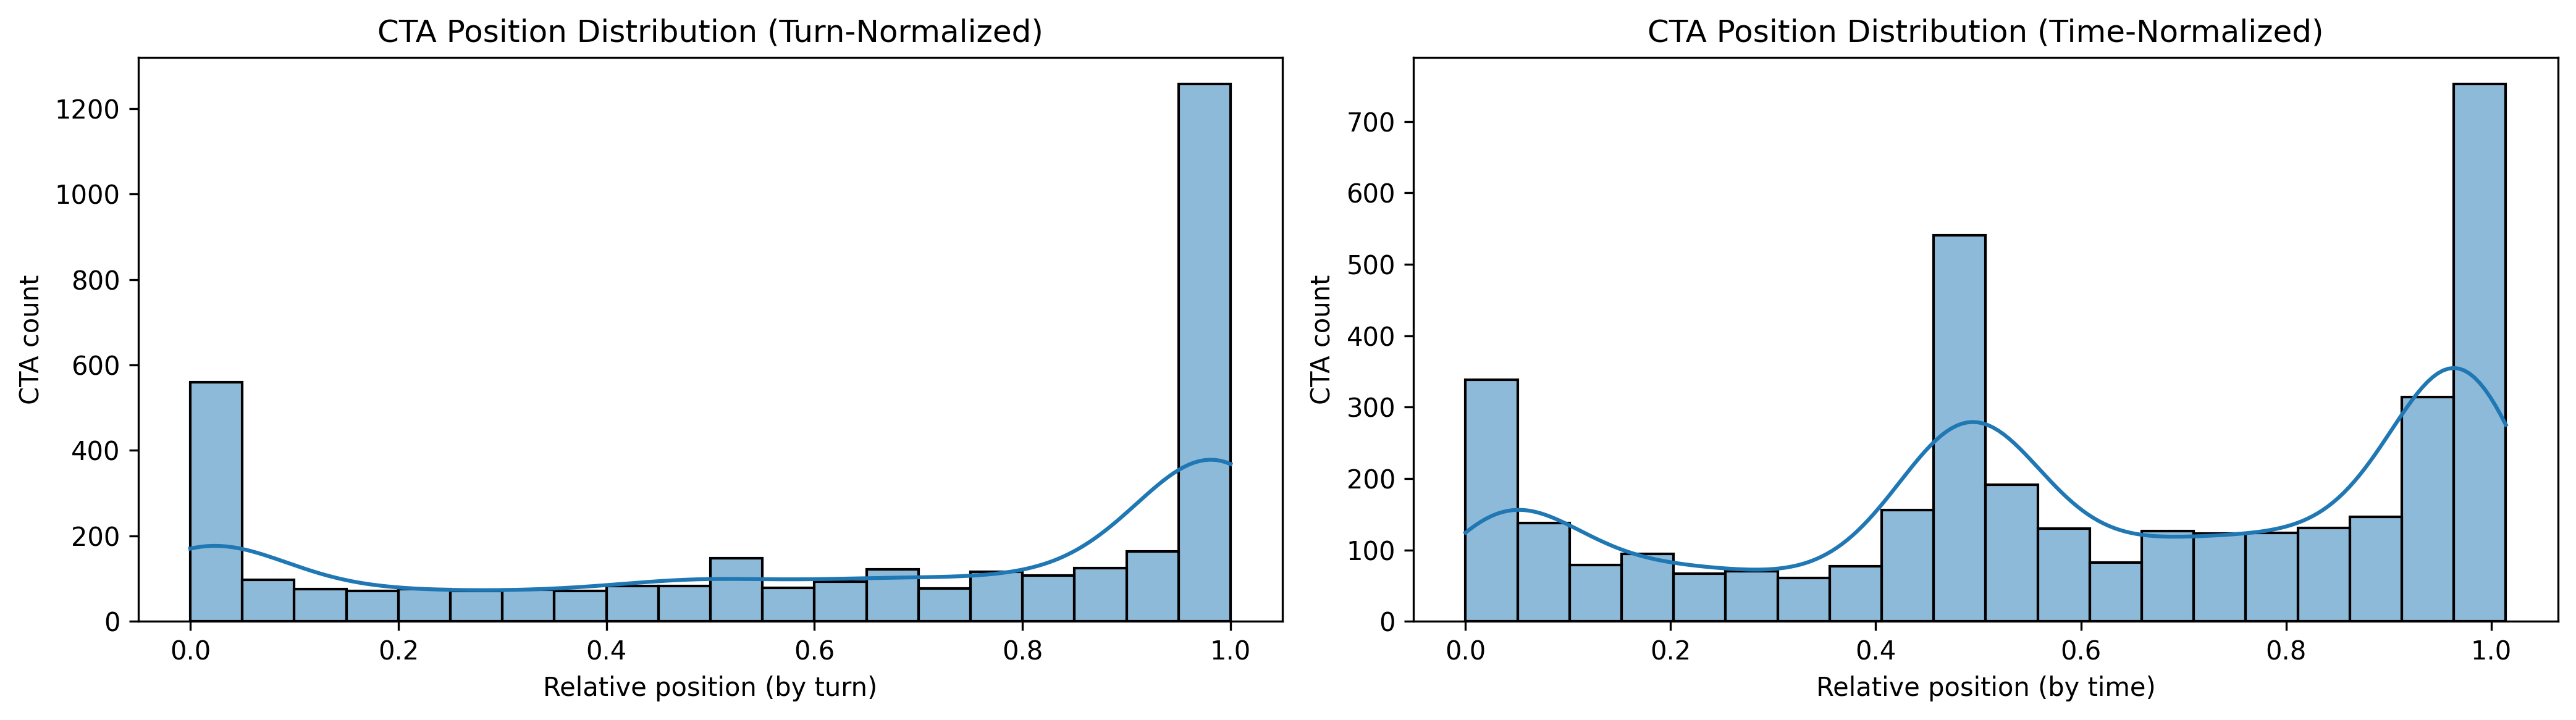
\includegraphics[width=\linewidth]{../figures/cta_position_turn_vs_time.png}
    \caption{Distribution of CTA positions within episodes under two normalization schemes. The left panel shows CTA locations normalized by turn index, while the right panel shows normalization by elapsed time. Turn based normalization produces a more diffuse distribution around the episode midpoint due to variation in turn length, whereas time based normalization yields clearer clustering near the beginning and end of episodes.}
    \label{fig:cta_position_turn_vs_time}
\end{figure}

\begin{figure}[h]
    \centering
    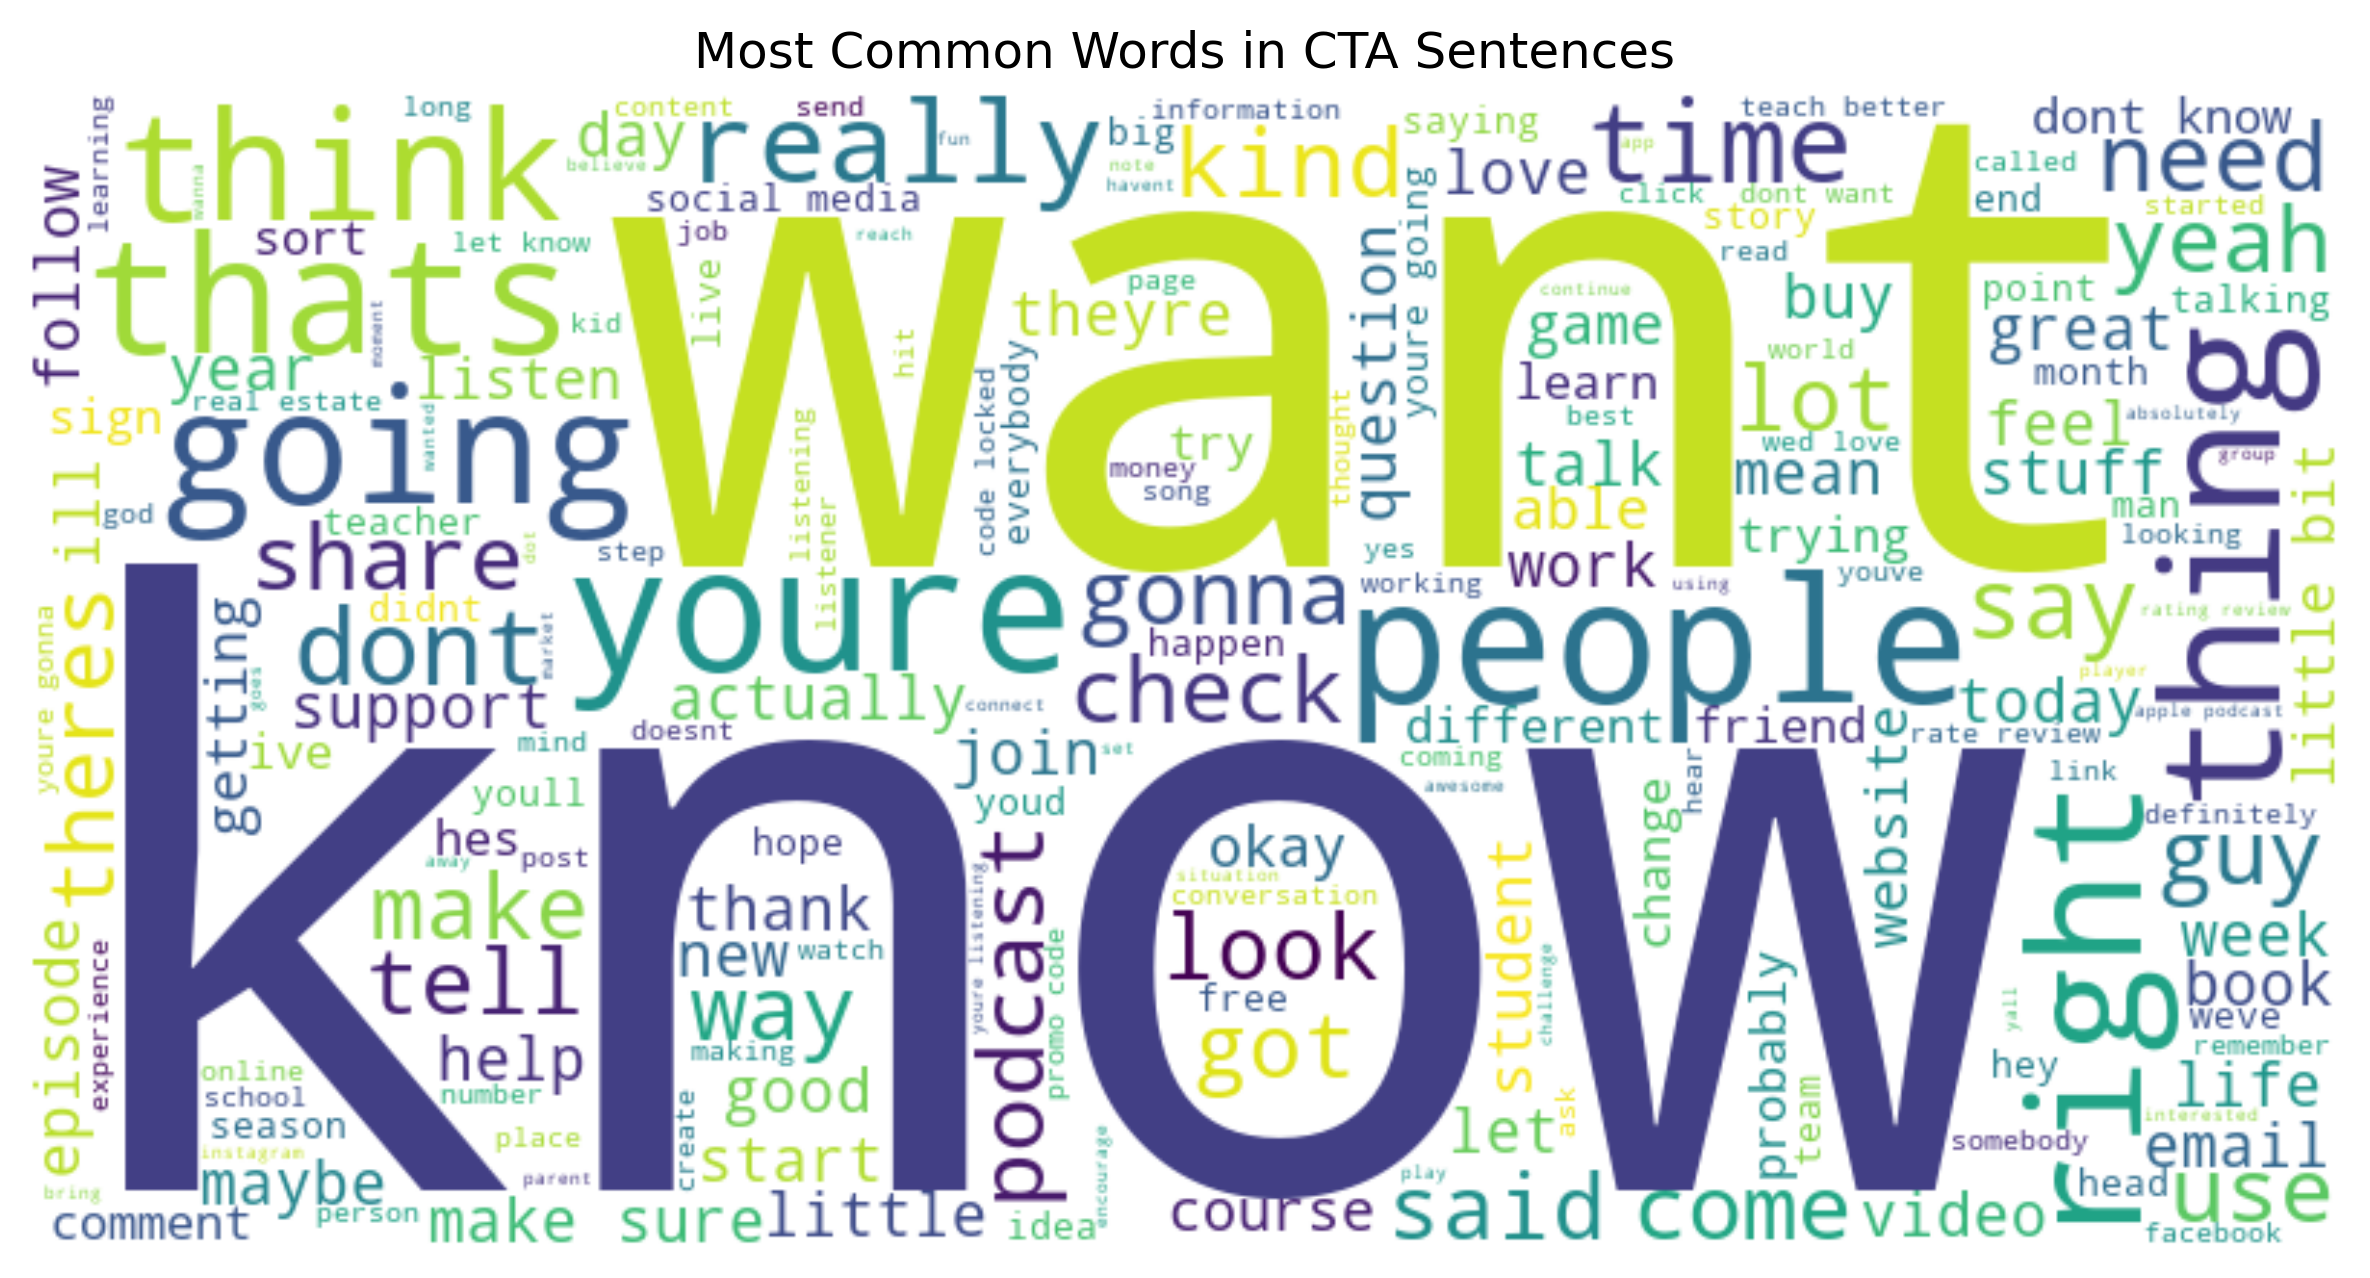
\includegraphics[width=0.8\linewidth]{../figures/cta_word_clould.png}
    \caption{Word cloud of the most frequent tokens in CTA sentences after applying stopword removal.}
    \label{fig:cta_word_cloud}
\end{figure}

\begin{figure}[h]
    \centering
    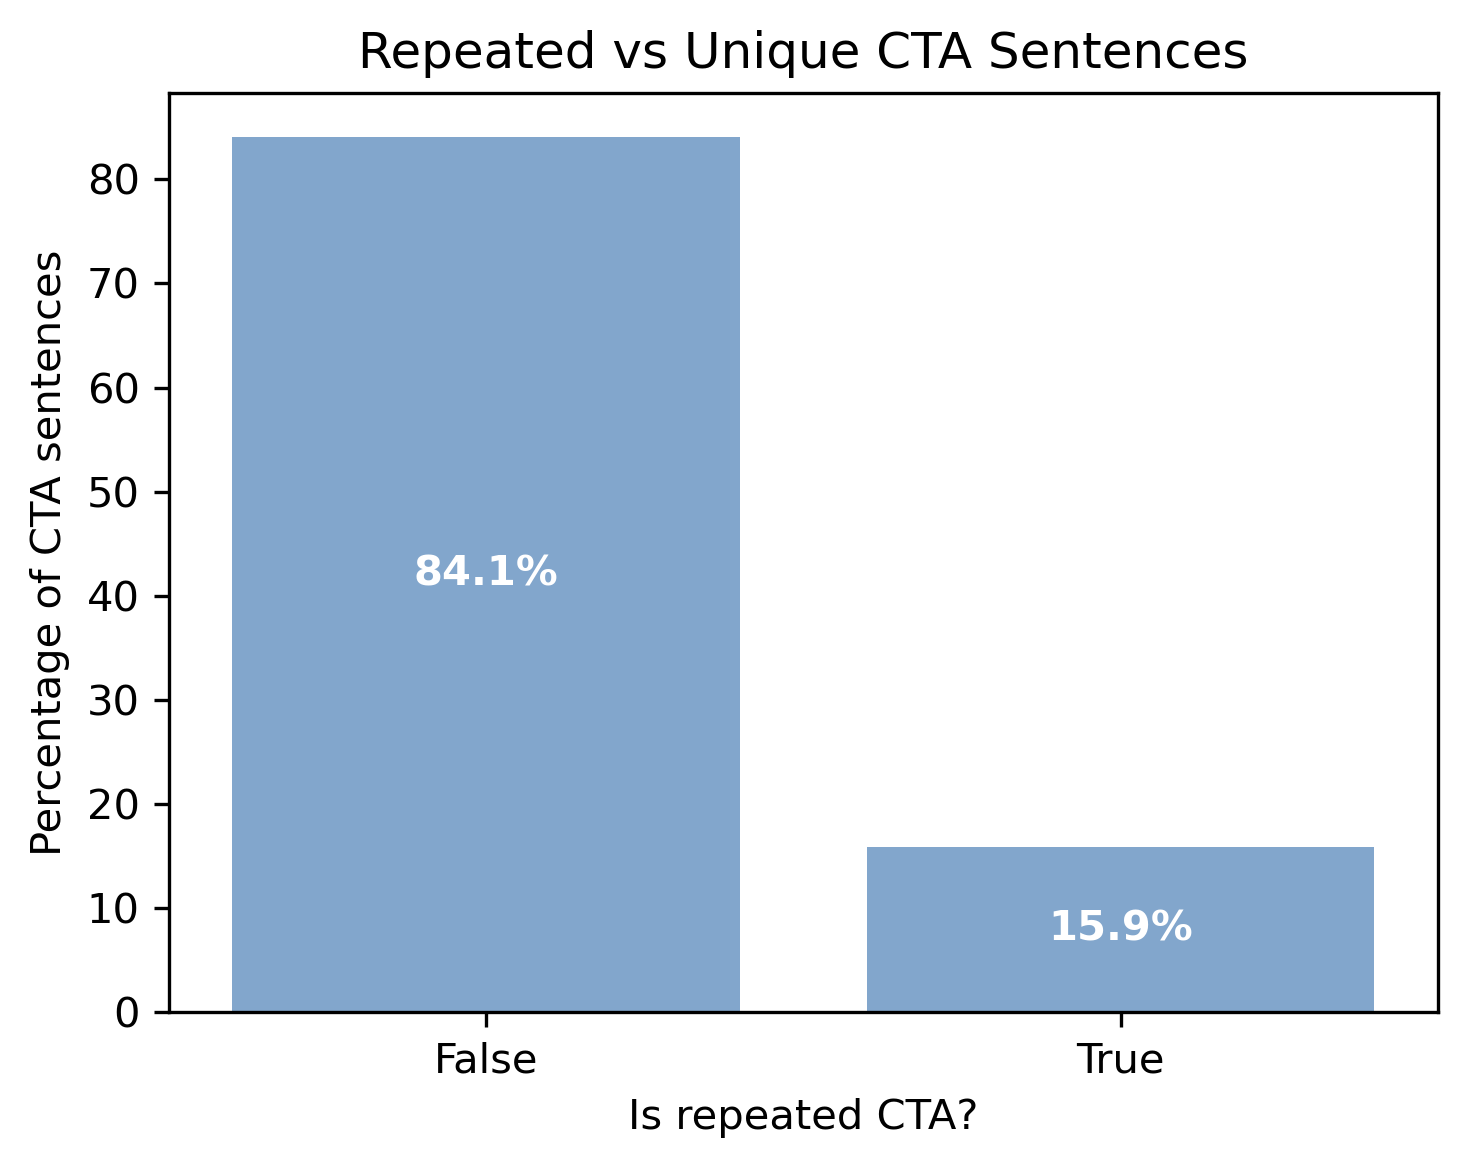
\includegraphics[width=0.7\linewidth]{../figures/cta_sent_repeats.png}
    \caption{Proportion of CTA sentences that are repeated versus unique after normalization. A non trivial share of CTA content consists of exact repeats, consistent with reused intro, outro, or sponsor scripts across episodes.}
    \label{fig:cta_sentence_repeats}
\end{figure}

\begin{figure}[h]
    \centering
    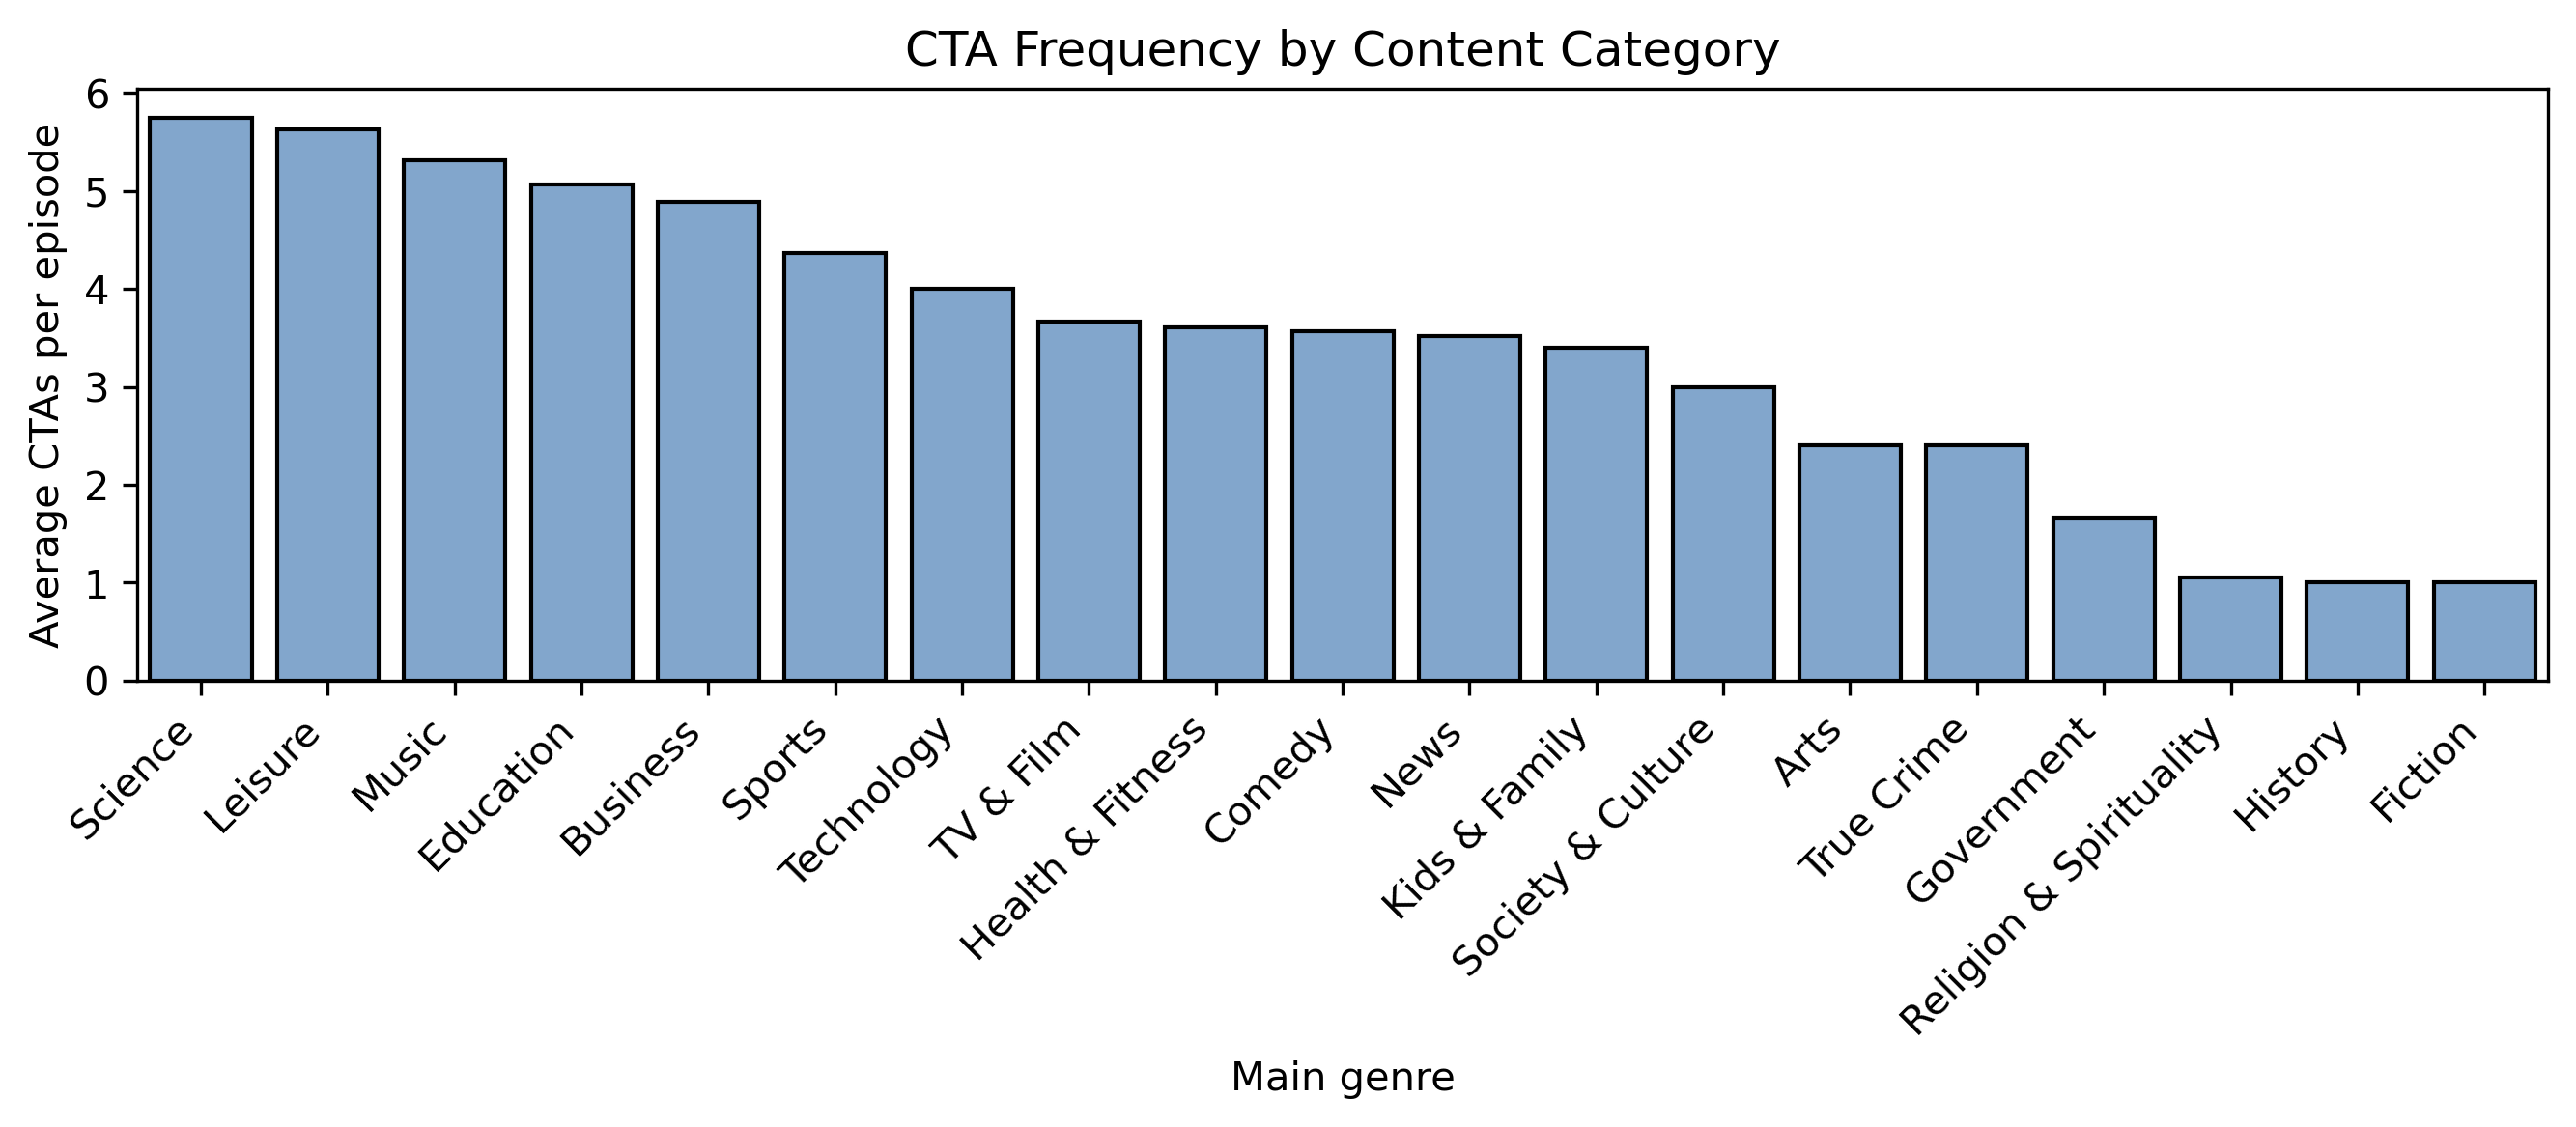
\includegraphics[width=\linewidth]{../figures/cta_freq_by_cat.png}
    \caption{Frequency of CTA occurrences across content categories. The distribution highlights systematic differences in how often calls to action are used across categories.}
    \label{fig:cta_frequency_by_category}
\end{figure}

\subsection{Interruption Figures}

\begin{figure}[h]
    \centering
    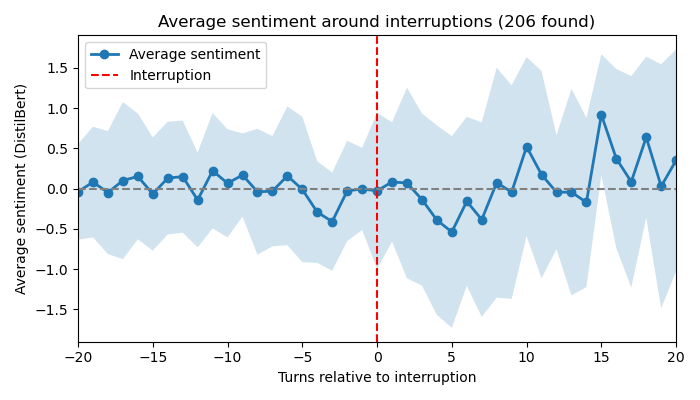
\includegraphics[width=\linewidth]{../figures/average_sentiment_demeaned_20.png}
    \caption{Average sentiment 20 turns before and after interruptions}
    \label{fig:sentiment_around_interruptions}
\end{figure}

\begin{figure}[h]
    \centering
    \includegraphics[width=\linewidth]{../figures/interuptions_by_category.png}
    \caption{Distribution of interruptions across genres on an episode level}
    \label{fig:interuptions_by_category}
\end{figure}

\begin{figure}[h]
    \centering
    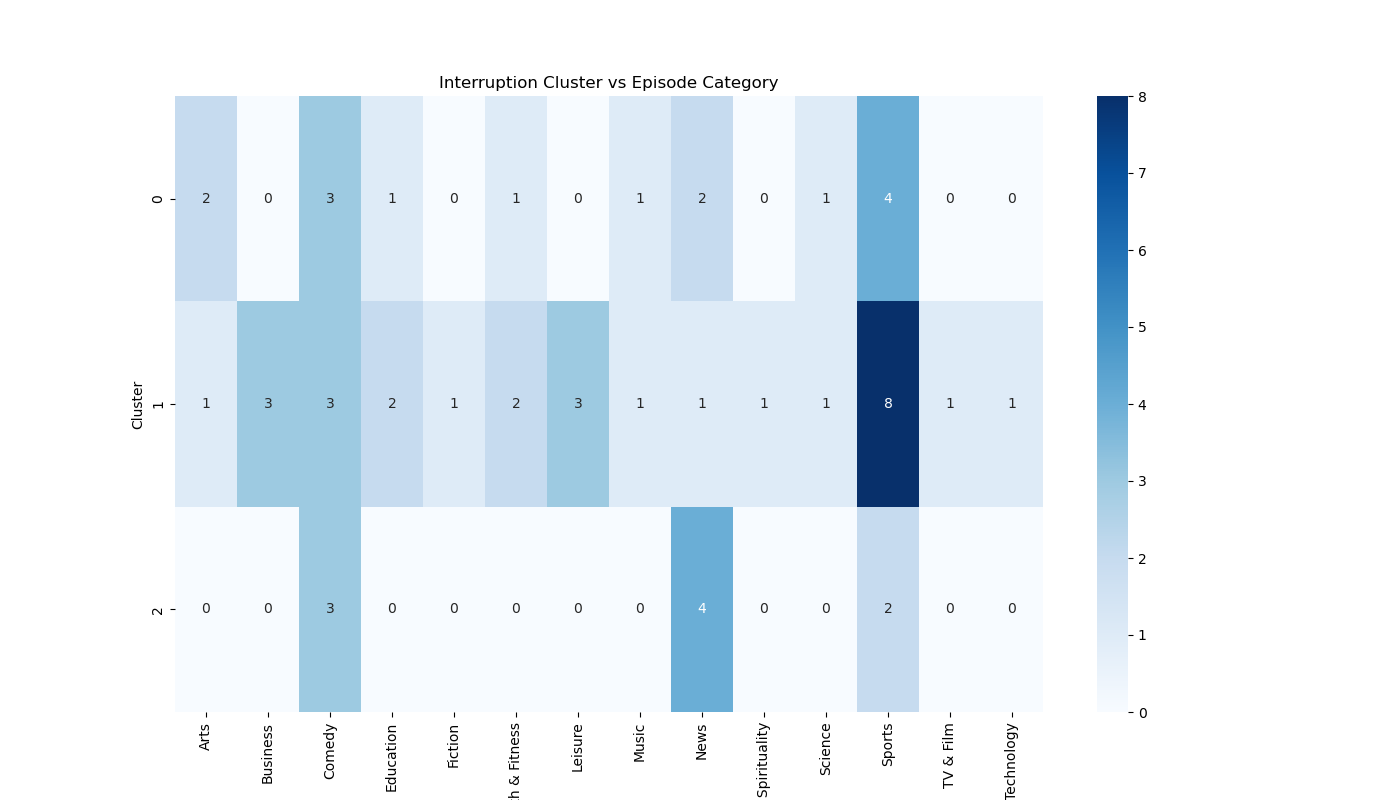
\includegraphics[width=\linewidth]{../figures/cluster_vs_category}
    \caption{Distribution of which clusters interruptions lie in across genres with K-means as the clustering method}
    \label{fig:cluster_vs_category}
\end{figure}

\end{document}
